\setcounter{section}{4} % This causes the next section to be Appendix B


\section*{Examples IV. 3D Time-dependent Behavior Examples}
\label{PS4}

This set of example problems is due on November 17, 2025. 

\medskip
\subsection*{4--1. \textbf{Characterization with deflection history} [4 pts].} 
A simply supported beam \textcolor{red}{with a uniform applied load (or you could instead use a point end load on a cantilevered beam as I mentioned on Slack, either is completely fine)} is made from a material that is well-described by a three-parameter standard linear solid model, i.e., the general creep compliance function $J_c(t)$ is given by
\begin{equation*}
    J_c(t) = J_\infty + (J_0 - J_\infty) \exp\left[-\frac{t}{\tau_c}\right],
\end{equation*}
where $J_\infty$, $J_0$, and $\tau_c$ are all mechanical properties of the material. 

The beam has a length of 4 ft and a second moment of area about the out-of-plane axis of 1 in$^4$. 
It is subjected to a position-time separable load function $q(z,t) = \hat{q}(z) \phi(t)$ where $\phi(t) = -3$ lb/ft $\cdot \mathcal{H}(t)$. 
Say we determine the maximum deflection in the beam at different times to be
\begin{align}
    &u_y \Big|_{\max} = -0.6 \textrm{~in~~at~~}t=30\textrm{~min}\\
    &u_y \Big|_{\max} = -0.75 \textrm{~in~at~~}t=60\textrm{~min}\\
    &u_y \Big|_{\max} = -1.0 \textrm{~in~~at~~}\textrm{~long times}
    \end{align}
From this, calibrate the material properties.

For an Euler--Bernoulli beam, the normal stress is related to the bending moment by
$$
\sigma_{xx}(y,t) = -\,\frac{y}{I}\,M(z,t),
$$
so, by linearity,
$$
\varepsilon_{xx}(y,t)
= -\,\frac{y}{I}\,\kappa(z,t),
$$
where $\kappa(z,t)$ is the curvature. Applying the same viscoelastic correspondence,
$$
\varepsilon_{xx}(y,t)
= \int_0^t J_c(t-\tau)\,\frac{\partial\sigma_{xx}(y,\tau)}{\partial\tau}\,d\tau
= -\,\frac{y}{I}\int_0^t J_c(t-\tau)\,\frac{\partial M(z,\tau)}{\partial\tau}\,d\tau.
$$
Comparing with $\varepsilon_{xx}(y,t) = -\dfrac{y}{I}\,\kappa(z,t)$, we obtain
$$
\kappa(z,t)
= \int_0^t J_c(t-\tau)\,\frac{\partial M(z,\tau)}{\partial\tau}\,d\tau.
$$

The load is
$$
q(z,t) = \hat{q}(z)\,\phi(t),
\qquad
\phi(t) = -3\,\mathrm{lb/ft}\cdot \mathcal{H}(t),
$$
Therefore,
$$
M(z,t) = \hat{M}(z)\,\phi(t)
= \hat{M}(z)\,q_0\,\mathcal{H}(t),
$$
with $q_0=-3\,\mathrm{lb/ft}$. Hence
$$
\frac{\partial M(z,\tau)}{\partial\tau}
= \hat{M}(z)\,q_0\,\delta(\tau),
$$
and the curvature becomes
$$
\kappa(z,t)
= \int_0^t J_c(t-\tau)\,\hat{M}(z)\,q_0\,\delta(\tau)\,d\tau
= \hat{M}(z)\,q_0\,J_c(t).
$$
So for a step load, the curvature field separates as
$$
\kappa(z,t) = J_c(t)\,\kappa_{\text{shape}}(z),
\qquad
\kappa_{\text{shape}}(z) := \hat{M}(z)\,q_0.
$$
Similarly, we can decompose
$$
u_y(z,t) = J_c(t)\,u_y^{\text{shape}}(z),
$$

At long times $t\to\infty$, the compliance tends to
$$
J_c(t) \to J_\infty,
$$
so
$$
u_{y,\max}(\infty) = u_{y, max}^{\text{shape}}(z)\,J_\infty.
$$
At any finite time,
$$
\frac{u_{y,\max}(t)}{u_{y,\max}(\infty)}
= \frac{J_c(t)}{J_\infty}
= \frac{J_\infty + (J_0-J_\infty)\exp(-t/\tau_c)}{J_\infty}
= 1 + \left(\frac{J_0}{J_\infty}-1\right)\exp\!\left(-\frac{t}{\tau_c}\right).
$$
Define the ratio
$$
r := \frac{J_0}{J_\infty},\qquad A := r-1.
$$

Using the given data:
$$
u_{y,\max}(30\ \mathrm{min}) = -0.6~\mathrm{in},
\quad
u_{y,\max}(60\ \mathrm{min}) = -0.75~\mathrm{in},
\quad
u_{y,\max}(\infty) = -1.0~\mathrm{in},
$$
we form the ratios
$$
\frac{0.6}{1.0} = 1 + A\,e^{-30/\tau_c},
\qquad
\frac{0.75}{1.0} = 1 + A\,e^{-60/\tau_c}.
$$
Thus
$$
-0.4 = A\,e^{-30/\tau_c},\qquad
-0.25 = A\,e^{-60/\tau_c}.
$$
Divide the second by the first:
$$
\frac{-0.25}{-0.4}
= \frac{e^{-60/\tau_c}}{e^{-30/\tau_c}}
\;\Rightarrow\;
0.625 = e^{-30/\tau_c}
\;\Rightarrow\;
\tau_c = -\frac{30}{\ln(0.625)} \approx 64~\mathrm{min}.
$$
Then
$$
A = \frac{-0.4}{e^{-30/\tau_c}} = \frac{-0.4}{0.625} = -0.64,
\qquad
r = 1 + A = 0.36.
$$
So
$$
\frac{J_0}{J_\infty} = 0.36
\quad\Rightarrow\quad
J_0 = 0.36\,J_\infty.
$$

To get absolute values, use the known long-time deflection.  
For a simply supported elastic beam with uniform load $q$:
$$
u_{y,\max}^{\text{elastic}} = -\frac{5 q L^4}{384\,E\,I}.
$$
In the viscoelastic step-load case, at long times $E$ is effectively replaced by $1/J_\infty$, giving
$$
u_{y,\max}(\infty) = -\frac{5 q L^4}{384\,I}\,J_\infty.
$$
With
$$
L = 4~\mathrm{ft} = 48~\mathrm{in},\quad
I = 1~\mathrm{in}^4,\quad
q = -3~\mathrm{lb/ft} = -0.25~\mathrm{lb/in},
$$
and $|u_{y,\max}(\infty)| = 1.0~\mathrm{in}$, we obtain
$$
J_\infty = \frac{384\,I}{5 |q| L^4}
\approx 5.8\times 10^{-5}\ \mathrm{in}^2/\mathrm{lb},
$$
and hence
$$
J_0 = 0.36\,J_\infty \approx 2.1\times 10^{-5}\ \mathrm{in}^2/\mathrm{lb}.
$$

\noindent\textbf{Final calibrated parameters:}
$$
J_0 \approx 2.1\times 10^{-5}\ \mathrm{in}^2/\mathrm{lb},
\qquad
J_\infty \approx 5.8\times 10^{-5}\ \mathrm{in}^2/\mathrm{lb},
\qquad
\tau_c \approx 64~\mathrm{min}.
$$

\bigskip
\subsection*{4--2. \textbf{Ramp up the torque} [4 pts].} 
A viscoelastic cylinder $AB$ is fixed on its end $A$ and simply supported on its opposite end at $B$. 
At point $B$, a second, rigid rod is joined to the end such that exerting a force on the rod will induce a counterclockwise torque about the axis of $AB$. 
A point force of magnitude $P_0$ is applied to the rigid rod, causing the front face to turn counterclockwise. 
The point force travels along the rod such that its distance from the bar's neutral axis $a(t)$ is direct in time, i.e., $a(t) = \alpha t$, where $\alpha$ is a constant. 
What is the angular rotation of the end $B$ as a function of time, $\Phi(t)$?

A point force $P_0$ acts at distance $a(t)=\alpha t$ from the cylinder axis, so the torque is
$$
T(t) = P_0\,a(t) = P_0\,\alpha\,t,\qquad t\ge 0.
$$
For a prismatic viscoelastic bar of length $L$ in torsion with shear creep compliance $J_c(t)$, the end rotation under a torque history $T(t)$ is
$$
\Phi(t) = \frac{L}{J_p}\int_0^t J_c(t-\tau)\,\frac{dT(\tau)}{d\tau}\,d\tau,
$$
where $J_p$ is the polar second moment of area.

Here
$$
\frac{dT}{d\tau} = P_0 \alpha \quad\text{(constant)},
$$
so
$$
\Phi(t) = \frac{L P_0 \alpha}{J_p}\int_0^t J_c(t-\tau)\,d\tau,
$$

\bigskip
\subsection*{4--3. \textbf{L-shaped beam} [4 pts].}
\begin{wrapfigure}[8]{r}{2in}
\vspace{-1cm}
    \centering
     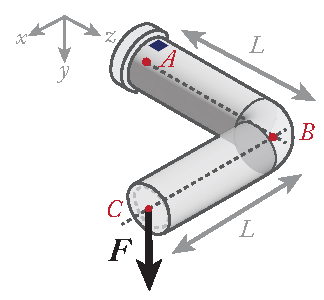
\includegraphics[scale=1]{instr-figures/L-bracket.pdf}
    \caption*{Figure 4.3a.}
    \label{fig:Lbracket}
\end{wrapfigure}
A one-piece polymeric member \textit{ABC} consists of two segments of length $L$ at a right angle from one-another and encastred at $A$, as shown. 
Its neutral axes both lie in the $x-z$ plane when unloaded. 
Assuming the creep compliance in shear to be $\mu_c(t)$ and the creep compliance in axial tension to be $E_c(t)$, determine (a) the deflection at $C$ in terms of the time-varying force $F(t)$ and (b) the stress tensor $\mathbf{\sigma}(t)$ at the square surface element located above $A$.

Let's first define the following quantities for a circular cross-section of radius $r$, area
$$
A = \pi r^2,
$$
second moment of area
$$
I = \frac{\pi r^4}{4},
$$
and torsional constant
$$
J = \frac{\pi r^4}{2},
$$

Because the load at $C$ produces:
\begin{itemize}
    \item bending in the horizontal leg $BC$, and
    \item torsion in the vertical leg $AB$,
\end{itemize}
the total deflection at $C$ is the sum of (i) bending of $BC$ and (ii) torsional rotation of $AB$,
converted into a transverse displacement.

% ---------------------------------------------------
\subsubsection*{(a) Deflection at $C$}

\paragraph{Bending of the segment $BC$}

The straight segment $BC$ behaves as a cantilever beam of length $L$ with a tip load $F(t)$.
The elastic benchmark for a cantilever with tip force $F$ is
$$
\delta_{\max}
=
\frac{F L^{3}}{3 E I}.
$$

To generalize this to a viscoelastic solid, we replace the elastic modulus $E$ by the
creep compliance $E_c(t)$ through the convolution form of Boltzmann superposition.
Thus, the bending deflection at $C$ is
$$
u_C^{(\text{bending})}(t)
=
\frac{L^{3}}{3 I}
\int_{0}^{t}
E_c(t-\tau)\,\frac{dF(\tau)}{d\tau}\,d\tau.
$$

% ---------------------------------------------------
\paragraph{Torsion of the segment $AB$}

The force at $C$ also produces a torque about the axis of segment $AB$.
The moment arm is the length $L$ of the horizontal segment $BC$, so the torque is
$$
T(t) = F(t)\,L.
$$

The correct elastic angle of twist for a circular prismatic bar is
$$
\phi = \frac{T L}{J G},
$$
where $J = \pi r^{4}/2$ is the torsional constant.

To generalize to a viscoelastic material using the shear creep compliance $\mu_c(t)$, we use  
Boltzmann superposition for torsion:
$$
\phi(t)
=
\frac{L^{2}}{J}
\int_{0}^{t}
\mu_c(t-\tau)\,\frac{dF(\tau)}{d\tau}\,d\tau.
$$

Point $C$, located at radius $r$ from the torsional axis, undergoes a transverse displacement
due to this rotation:
$$
u_C^{(\text{torsion})}(t)
=
r \,\phi(t)
=
\frac{r L^{2}}{J}
\int_{0}^{t}
\mu_c(t-\tau)\,\frac{dF(\tau)}{d\tau}\,d\tau.
$$


% ---------------------------------------------------
\paragraph{Total deflection at $C$}

The deflection of point $C$ is the sum of bending of the horizontal segment and the torsional
rotation of the vertical segment:
$$
u_C(t)
=
\frac{L^{3}}{3 I}
\int_{0}^{t}
E_c(t-\tau)\,\frac{dF(\tau)}{d\tau}\,d\tau
+
\frac{r L^{2}}{J}
\int_{0}^{t}
\mu_c(t-\tau)\,\frac{dF(\tau)}{d\tau}\,d\tau.
$$

% ---------------------------------------------------
\subsubsection*{(b) Stress tensor at the square surface above $A$}

We work in a local orthonormal basis attached to the segment $AB$:
$$
\bm{e}_1 \text{ along the z axis},\quad
\bm{e}_2 \text{ along the -y axis},\quad
\bm{e}_3 = \bm{e}_1 \times \bm{e}_2.
$$

The internal resultants at the fixed end $A$ due to the tip force $F(t)$ are, for this
L-shaped bracket,
$$
V(t) = F(t), \qquad
M(t) = F(t)\,L, \qquad
T(t) = F(t)\,L,
$$

\begin{itemize}
  \item \textbf{Normal (bending) stress} at a point a distance $y$ from the neutral axis
  in the $\bm{e}_2$ direction:
  $$
  \sigma_{11}^{(\text{bend})}(t)
  = -\,\frac{M(t)\,y}{I}.
  $$
  At the outer fiber of the surface element above $A$ we have $y = r$, so
  $$
  \sigma_{11}^{(\text{bend})}(t)
  = -\,\frac{F(t)\,L\,r}{I}.
  $$

  \item \textbf{Shear stress from torsion} at radius $r$ in the $\bm{e}_3$ (circumferential)
  direction:
  $$
  \tau_{13}^{(\text{torsion})}(t)
  = \frac{T(t)\,r}{J}
  = \frac{F(t)\,L\,r}{J}.
  $$

  \item \textbf{Shear stress from transverse F} at point A in the $\bm{e}_2$ direction:
  $$
  \tau_{12}^{(\text{transverse force})}(t)
  = \frac{V(t)\,Q}{It}
  = 0.
  $$
  , as $Q$ is 0 at the surface.
\end{itemize}

The non-zero components of the Cauchy stress tensor in the
local basis $\{\bm{e}_1,\bm{e}_2,\bm{e}_3\}$ at the outer surface point are
$$
\sigma_{11}(t) = -\,\frac{F(t)\,L\,r}{I}, \qquad
\sigma_{13}(t) = \sigma_{31}(t) = \frac{F(t)\,L\,r}{J}.
$$

Thus the stress tensor can be written as
$$
\bm{\sigma}(t)
=
\sigma_{11}(t)\,\bm{e}_1\otimes\bm{e}_1
+
\tau_{13}(t)\,\big(
\bm{e}_1\otimes\bm{e}_3
+
\bm{e}_3\otimes\bm{e}_1
\big)
$$

\newpage
\subsection*{4--4. \textbf{Fibrous material} [4 pts].}
An elastic material with a fiber phase has the Helmholtz free energy function
\begin{equation*}
\widetilde{\psi}(\bn{F}) = \frac{1}{2}C_{10} (I_1-3) + \frac{1}{4} k (I_a - 1)^2,
\end{equation*}
where $I_1(\bn{C}) = \textrm{tr}(\bn{C})$ and $I_a(\bn{C},\hat{\bm{a}}_0) = \hat{\bm{a}}_0 \cdot \bn{C} \hat{\bm{a}}_0$ for $\bn{C} = \bn{F}^\intercal \bn{F}$.

%\skiponeline
%(a) Show that, given the direction $\hat{\bm{a}}_0$ is fixed by the material, $I_a$ is an invariant of $\bn{C}$.

\medskip
(a) Show that this elastic potential is consistent with the principle of objectivity.

A superposed rigid rotation $\mathbf{Q}\in\mathrm{SO}(3)$ gives
$$
\mathbf{F}^\ast=\mathbf{Q}\mathbf{F},\qquad
\mathbf{C}^\ast=(\mathbf{F}^\ast)^\top\mathbf{F}^\ast
=\mathbf{F}^\top\mathbf{Q}^\top\mathbf{Q}\mathbf{F}
=\mathbf{F}^\top\mathbf{F}=\mathbf{C}.
$$
Thus
$$
I_1(\mathbf{C}^\ast)=I_1(\mathbf{C}),\qquad
I_a(\mathbf{C}^\ast,\hat{\mathbf{a}}_0)=\hat{\mathbf{a}}_0\cdot\mathbf{C}^\ast\hat{\mathbf{a}}_0
=\hat{\mathbf{a}}_0\cdot\mathbf{C}\hat{\mathbf{a}}_0=I_a(\mathbf{C},\hat{\mathbf{a}}_0),
$$
because $\hat{\mathbf{a}}_0$ is fixed in the material (reference) frame. Hence
$$
\widetilde{\psi}(\mathbf{Q}\mathbf{F})=\widetilde{\psi}(\mathbf{F}),
$$
so the potential is objective.

\medskip
(b) Show that the material symmetry group $\mathcal{G}$ is the set of all proper orthogonal tensors $\bn{H}$ with $\bn{H}\hat{\bm{a}}_0 = \hat{\bm{a}}_0$.  

A right symmetry $\mathbf{H}$ must satisfy
$$
\widetilde{\psi}(\mathbf{F}\mathbf{H})=\widetilde{\psi}(\mathbf{F})\quad\forall\,\mathbf{F}.
$$
For $\mathbf{F}\mathbf{H}$,
$$
\mathbf{C}'=(\mathbf{F}\mathbf{H})^\top (\mathbf{F}\mathbf{H})
=\mathbf{H}^\top \mathbf{C}\,\mathbf{H}.
$$
Then
$$
I_1(\mathbf{C}')=\mathrm{tr}(\mathbf{H}^\top \mathbf{C}\mathbf{H})
=\mathrm{tr}(\mathbf{C}\mathbf{H}\mathbf{H}^\top)=\mathrm{tr}\,\mathbf{C}=I_1(\mathbf{C}),
$$
for any $\mathbf{H}\in\mathrm{SO}(3)$.
For $I_a$,
$$
I_a'=\hat{\mathbf{a}}_0\cdot\mathbf{C}'\hat{\mathbf{a}}_0
=\hat{\mathbf{a}}_0\cdot\mathbf{H}^\top \mathbf{C}\mathbf{H}\hat{\mathbf{a}}_0
=(\mathbf{H}\hat{\mathbf{a}}_0)\cdot\mathbf{C}(\mathbf{H}\hat{\mathbf{a}}_0).
$$
For $I_a'=I_a$ for \emph{all} $\mathbf{C}$, we require
$$
\mathbf{H}\hat{\mathbf{a}}_0 = \hat{\mathbf{a}}_0.
$$
Thus the material symmetry group is
$$
\displaystyle
\mathcal{G}
=\left\{\mathbf{H}\in\mathrm{SO}(3)\ \big|\ \mathbf{H}\hat{\mathbf{a}}_0=\hat{\mathbf{a}}_0\right\},
$$
i.e. all rotations about the fiber direction $\hat{\mathbf{a}}_0$ (transverse isotropy).

\medskip
(c) Find the first Piola-Kirchhoff and Cauchy stress expressions with an applied deformation gradient tensor of $\bn{F}$.

First compute
$$
\frac{\partial I_1}{\partial\mathbf{C}}=\mathbf{I},\qquad
\frac{\partial I_a}{\partial\mathbf{C}}=\hat{\mathbf{a}}_0\otimes\hat{\mathbf{a}}_0.
$$
Then
$$
\frac{\partial\widetilde{\psi}}{\partial\mathbf{C}}
= \frac12 C_{10}\,\mathbf{I}
+ \frac14 k\cdot 2(I_a-1)(\hat{\mathbf{a}}_0\otimes\hat{\mathbf{a}}_0)
= \frac12 C_{10}\,\mathbf{I}
+ \frac12 k(I_a-1)(\hat{\mathbf{a}}_0\otimes\hat{\mathbf{a}}_0).
$$
So the second Piola–Kirchhoff stress is
$$
\mathbf{S} = 2\,\frac{\partial\widetilde{\psi}}{\partial\mathbf{C}}
= C_{10}\,\mathbf{I}+k(I_a-1)(\hat{\mathbf{a}}_0\otimes\hat{\mathbf{a}}_0).
$$

The first Piola–Kirchhoff stress is
$$
\displaystyle
\mathbf{P} = \mathbf{F}\,\mathbf{S}
= \mathbf{F}\Big[ C_{10}\,\mathbf{I}+k(I_a-1)(\hat{\mathbf{a}}_0\otimes\hat{\mathbf{a}}_0)\Big].
$$

Let
$$
\mathbf{a} = \mathbf{F}\hat{\mathbf{a}}_0,\qquad
\mathbf{B}=\mathbf{F}\mathbf{F}^\top,\qquad
J=\det\mathbf{F}.
$$
The Cauchy stress is
$$
\boldsymbol{\sigma} = \frac{1}{J}\,\mathbf{P}\mathbf{F}^\top
= \frac{1}{J}\Big[C_{10}\,\mathbf{B}
+ k(I_a-1)(\mathbf{a}\otimes\mathbf{a})\Big].
$$

For an incompressible material ($J=1$) with Lagrange multiplier $p$, it should be added $-p\mathbf{I}$:
$$
\displaystyle
\boldsymbol{\sigma}
= C_{10}\,\mathbf{B}
+ k(I_a-1)(\mathbf{a}\otimes\mathbf{a})
- p\,\mathbf{I}.
$$

\bigskip
\bigskip
\subsection*{4--5. \textbf{Gent model of rubber elasticity} [4 pts].}
The Gent model, which incorporates the finite extensibility of polymer chains in a rubber network but includes $I_2$-dependence, has a\textcolor{red}{n isochoric} free-energy function of $$\bar{\Psi}_{\textcolor{red}{\textrm{iso}}} = -\frac{C_{10}}{2} J_m \ln \left(1 - \frac{I_1-3}{J_m} \right) + C_{01}\ln \left(\frac{I_2}{3}\right), $$ where $C_{10}>0$, $C_{01}\geq 0$, and $J_m>0$ are material constants.

\medskip
(a) Show that the Cauchy stress corresponding to the free energy above has the form\footnote{\textcolor{red}{You may want to use the Cayley-Hamilton theorem to do a replacement for $\bn{B}^2$, which produces $\bn{B}^2 = I_1 \bn{B} - I_2 \bn{I} + I_3 \bn{B}^{-1}$.}} $$\bm{\sigma} = -p \bn{I} + \frac{C_{10} J_m}{J_m - (I_1-3)}\bn{B} - \frac{2C_{01}}{I_2} \bn{B}^{-1}.$$

For an incompressible isotropic solid, the Cauchy stress is
$$
\boldsymbol{\sigma}
= -p\,\mathbf{I}
+ 2\frac{\partial\bar{\Psi}_{\mathrm{iso}}}{\partial I_1}\mathbf{B}
- 2\frac{\partial\bar{\Psi}_{\mathrm{iso}}}{\partial I_2}\mathbf{B}^{-1},
$$

Compute
$$
\frac{\partial\bar{\Psi}_{\mathrm{iso}}}{\partial I_1}
= -\frac{C_{10}}{2}J_m\cdot
\frac{1}{1-\frac{I_1-3}{J_m}}\left(-\frac{1}{J_m}\right)
= \frac{C_{10}}{2}\frac{J_m}{J_m-(I_1-3)},
$$
and
$$
\frac{\partial\bar{\Psi}_{\mathrm{iso}}}{\partial I_2}
= C_{01}\cdot\frac{1}{I_2}.
$$
Therefore
$$
\boldsymbol{\sigma}
= -p\,\mathbf{I}
+ 2\left(\frac{C_{10}}{2}\frac{J_m}{J_m-(I_1-3)}\right)\mathbf{B}
- 2\left(\frac{C_{01}}{I_2}\right)\mathbf{B}^{-1},
$$
so
$$
\displaystyle
\boldsymbol{\sigma}
= -p\,\mathbf{I}
+ \frac{C_{10}J_m}{J_m-(I_1-3)}\,\mathbf{B}
- \frac{2C_{01}}{I_2}\,\mathbf{B}^{-1}.
$$

\medskip
(b) This material undergoes a simple shear deformation of magnitude $\gamma$. Given that the shear modulus $\mu(\gamma^2) \equiv \beta_1(\gamma^2) - \beta_{-1} (\gamma^2)$ where $\beta_i$ corresponds to the expression for $\bm{\sigma}$ in Q1, show that in the small strain limit that $$\lim\limits_{\gamma \rightarrow 0} \mu(\gamma^2) = C_{10} + \frac{2}{3} C_{01}.$$

Consider simple shear of magnitude $\gamma$:
$$
\mathbf{F} =
\begin{pmatrix}
1 & \gamma & 0\\
0 & 1 & 0\\
0 & 0 & 1
\end{pmatrix},
\qquad
\mathbf{B}=\mathbf{F}\mathbf{F}^\top
=
\begin{pmatrix}
1+\gamma^2 & \gamma & 0\\
\gamma & 1 & 0\\
0 & 0 & 1
\end{pmatrix}.
$$
Then
$$
I_1 = 3+\gamma^2,\qquad
I_2 = 3+\gamma^2
$$
for this deformation.

We can write the Cauchy stress in the standard representation
$$
\boldsymbol{\sigma}
= -p\,\mathbf{I}
+ \beta_1(\gamma^2)\,\mathbf{B}
- \beta_{-1}(\gamma^2)\,\mathbf{B}^{-1},
$$
where, by comparison with part (a),
$$
\beta_1(\gamma^2) = \frac{C_{10}J_m}{J_m-(I_1-3)}
= \frac{C_{10}J_m}{J_m-\gamma^2},
\qquad
\beta_{-1}(\gamma^2) = \frac{2C_{01}}{I_2}
= \frac{2C_{01}}{3+\gamma^2}.
$$

Evaluate at $\gamma=0$:
$$
\beta_1(0) = \frac{C_{10}J_m}{J_m} = C_{10},\qquad
\beta_{-1}(0) = \frac{2C_{01}}{3}.
$$
So
$$
\displaystyle
\lim_{\gamma\to 0}\mu(\gamma^2)
= C_{10}+\frac{2}{3}C_{01}.
$$